\documentclass[aspectratio=169]{beamer}

\usetheme{Boadilla}
\usefonttheme{professionalfonts}
\setbeamertemplate{navigation symbols}{}
\setbeamertemplate{itemize items}[circle]
\setbeamertemplate{enumerate items}[default]
\setbeamertemplate{headline}{}

\usepackage[utf8]{inputenc}
\usepackage[T1]{fontenc}
\usepackage{lmodern}
\usepackage{amsmath}
\usepackage{booktabs}
\usepackage{tabularx}
\usepackage{array}
\usepackage{hyperref}
\usepackage[strings]{underscore}
\usepackage{listings}
\usepackage{tikz}
\usetikzlibrary{arrows.meta,positioning,fit,calc,shapes.geometric}
\usepackage{xcolor}

\definecolor{courseblue}{HTML}{12355B}
\definecolor{coursegold}{HTML}{C98A2E}
\definecolor{courseice}{HTML}{EEF3F8}
\definecolor{coursegreen}{HTML}{2F6B4F}
\definecolor{coursegray}{HTML}{4B5563}
\definecolor{codebg}{HTML}{F7F9FC}
\definecolor{codecomment}{HTML}{5E6C84}
\definecolor{codestring}{HTML}{0B6E4F}

\setbeamercolor{palette primary}{bg=courseblue,fg=white}
\setbeamercolor{palette secondary}{bg=coursegold,fg=white}
\setbeamercolor{palette tertiary}{bg=courseblue,fg=white}
\setbeamercolor{palette quaternary}{bg=coursegold,fg=white}
\setbeamercolor{structure}{fg=courseblue}
\setbeamercolor{frametitle}{bg=courseice,fg=courseblue}
\setbeamercolor{title}{fg=courseblue}
\setbeamercolor{block title}{bg=courseblue,fg=white}
\setbeamercolor{block body}{bg=courseice,fg=black}
\setbeamercolor{normal text}{fg=black,bg=white}
\setbeamercolor{alerted text}{fg=coursegold}

\setbeamerfont{footline}{size=\scriptsize}

\setbeamertemplate{footline}{
  \leavevmode
  \hbox{
    \begin{beamercolorbox}[wd=.33\paperwidth,ht=2.8ex,dp=1.2ex,leftskip=0.8em]{palette primary}%
      University of Trieste
    \end{beamercolorbox}%
    \begin{beamercolorbox}[wd=.49\paperwidth,ht=2.8ex,dp=1.2ex,center]{palette tertiary}%
      \coursename{} \textbar{} \coursecode
    \end{beamercolorbox}%
    \begin{beamercolorbox}[wd=.18\paperwidth,ht=2.8ex,dp=1.2ex,rightskip=0.8em plus1fil]{palette secondary}%
      \insertframenumber{} / \inserttotalframenumber
    \end{beamercolorbox}%
  }
}

\hypersetup{
  colorlinks=true,
  linkcolor=courseblue,
  urlcolor=coursegreen
}

\lstdefinestyle{coursepython}{
  language=Python,
  basicstyle=\ttfamily\footnotesize,
  keywordstyle=\color{courseblue}\bfseries,
  commentstyle=\color{codecomment}\itshape,
  stringstyle=\color{codestring},
  showstringspaces=false,
  columns=fullflexible,
  keepspaces=true,
  frame=single,
  framerule=0.6pt,
  rulecolor=\color{courseblue},
  backgroundcolor=\color{codebg},
  xleftmargin=0.4em,
  xrightmargin=0.4em,
  aboveskip=0.4em,
  belowskip=0.2em
}

\newcommand{\coursename}{Data-driven Systems Engineering}
\newcommand{\coursecode}{440MI / 305SM}
\newcommand{\coursefooter}{}

\newcommand{\learninggoals}[1]{
  \begin{block}{Learning goals}
  #1
  \end{block}
}

\newcommand{\repoactivity}[1]{
  \begin{block}{Repo activity}
  #1
  \end{block}
}

\newcommand{\readinglist}[1]{
  \begin{block}{Papers and materials}
  {\footnotesize #1}
  \end{block}
}

\newcommand{\coursecontextframe}[5]{
  \begin{frame}{Course Map and Running Cases}
  \centering
  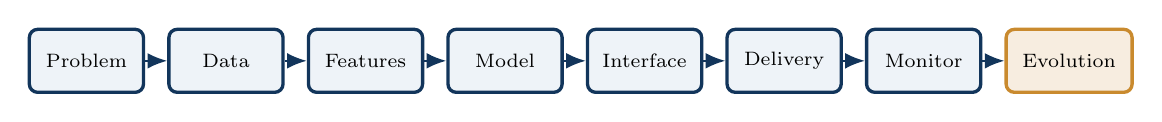
\begin{tikzpicture}[node distance=0.28cm]
  \node[flowbox, minimum width=1.45cm, minimum height=0.8cm] (problem) {\scriptsize Problem};
  \node[flowbox, minimum width=1.45cm, minimum height=0.8cm, right=of problem] (data) {\scriptsize Data};
  \node[flowbox, minimum width=1.45cm, minimum height=0.8cm, right=of data] (features) {\scriptsize Features};
  \node[flowbox, minimum width=1.45cm, minimum height=0.8cm, right=of features] (model) {\scriptsize Model};
  \node[flowbox, minimum width=1.45cm, minimum height=0.8cm, right=of model] (interface) {\scriptsize Interface};
  \node[flowbox, minimum width=1.45cm, minimum height=0.8cm, right=of interface] (delivery) {\scriptsize Delivery};
  \node[flowbox, minimum width=1.45cm, minimum height=0.8cm, right=of delivery] (monitor) {\scriptsize Monitor};
  \node[accentbox, minimum width=1.6cm, minimum height=0.8cm, right=of monitor] (evolution) {\scriptsize Evolution};
  \foreach \a/\b in {problem/data,data/features,features/model,model/interface,interface/delivery,delivery/monitor,monitor/evolution} {
    \draw[arrow] (\a) -- (\b);
  }
  \end{tikzpicture}

  \vspace{0.5em}
  \begin{block}{Today in the course}
  \textbf{Focus:} #1

  \textbf{Bridge:} #2
  \end{block}

  \begin{columns}[T]
  \column{0.48\textwidth}
  \begin{block}{Fraud case}
  {\footnotesize #3}
  \end{block}
  \column{0.48\textwidth}
  \begin{block}{Pasteurization case}
  {\footnotesize #4}
  \end{block}
  \end{columns}

  \vspace{0.3em}
  {\footnotesize \textbf{Course thread:} #5}
  \coursefooter
  \end{frame}
}

\newcommand{\classclosingframe}[4]{
  \begin{frame}{From This Class to the Next}
  \begin{block}{What stays with us}
  #1
  \end{block}

  \begin{columns}[T]
  \column{0.48\textwidth}
  \begin{block}{Project use}
  {\footnotesize #2}
  \end{block}
  \column{0.48\textwidth}
  \begin{block}{Next connection}
  {\footnotesize #3}
  \end{block}
  \end{columns}

  \vspace{0.3em}
  {\footnotesize \textbf{Course thread:} #4}
  \coursefooter
  \end{frame}
}

\tikzset{
  flowbox/.style={
    rounded corners=3pt,
    draw=courseblue,
    fill=courseice,
    very thick,
    minimum width=2.2cm,
    minimum height=0.9cm,
    align=center,
    font=\small
  },
  accentbox/.style={
    rounded corners=3pt,
    draw=coursegold,
    fill=coursegold!15,
    very thick,
    minimum width=2.2cm,
    minimum height=0.9cm,
    align=center,
    font=\small
  },
  arrow/.style={
    -{Latex[length=2.5mm,width=2mm]},
    thick,
    draw=courseblue
  }
}


\title{Class 30: Good Practices with Docker and CI/CD}
\subtitle{Session 30 of 36 -- MLOps Block}
\author{\coursename}
\date{}

\begin{document}

\frame{\titlepage \coursefooter}

\begin{frame}{Agenda}
\begin{itemize}
\item Why delivery pipelines matter for ML systems.
\item Docker and GitHub Actions in the course workflow.
\item Pipeline stages, gates, and release safety.
\item What to test before deployment.
\item Repository examples from the Flask and Streamlit apps.
\item Reproducibility, release safety, and rollback thinking.
\end{itemize}
\coursefooter
\end{frame}

\begin{frame}{Why good delivery practice deserves its own class}
\learninggoals{
\begin{itemize}
\item Understand how packaging and automation reduce deployment friction.
\item Connect notebooks and services to Docker and GitHub Actions.
\item Learn what should be tested before a model-backed service is released.
\item Explain why CI/CD in ML must validate both software and artifacts.
\end{itemize}
}
\coursefooter
\end{frame}

\coursecontextframe
{Packaging, testing, and automated delivery.}
{This class moves the course from local development into repeatable release processes that reduce deployment risk.}
{In the fraud case, the scoring service becomes containerized, testable, and suitable for CI-driven release checks.}
{In the pasteurization case, dashboards and streaming services gain a repeatable environment so demonstrations do not depend on one laptop state.}
{The key course shift is from building a system to proving that it can be rebuilt and shipped consistently.}

\begin{frame}{A delivery pipeline is a risk-control mechanism}
\begin{itemize}
\item CI/CD is not only about speed. Its main purpose is to make releases safer and more repeatable.
\item In ML systems, the release unit often includes code, dependencies, configuration, and trained artifacts.
\item A pipeline reduces the number of assumptions hidden inside one developer machine.
\end{itemize}
\coursefooter
\end{frame}

\begin{frame}{From local success to repeatable delivery}
\centering
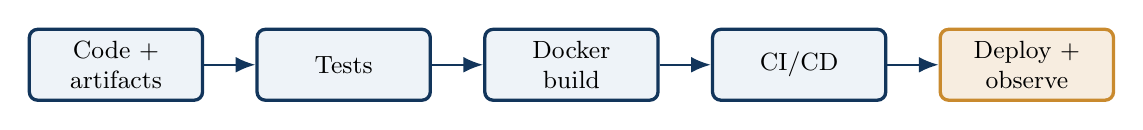
\begin{tikzpicture}[node distance=0.7cm and 0.65cm]
\node[flowbox] (code) {Code +\\artifacts};
\node[flowbox, right=of code] (test) {Tests};
\node[flowbox, right=of test] (docker) {Docker\\build};
\node[flowbox, right=of docker] (ci) {CI/CD};
\node[accentbox, right=of ci] (deploy) {Deploy +\\observe};
\draw[arrow] (code) -- (test);
\draw[arrow] (test) -- (docker);
\draw[arrow] (docker) -- (ci);
\draw[arrow] (ci) -- (deploy);
\end{tikzpicture}
\vspace{0.7em}
\begin{itemize}
\item Deterministic installs and smoke tests should happen before container release.
\item Deployment is not the end; health checks and logs are part of the pipeline.
\end{itemize}
\coursefooter
\end{frame}

\begin{frame}{Why ML delivery is harder than standard app delivery}
\begin{itemize}
\item The build may depend on large artifacts that are not regenerated on every commit.
\item A working container can still be wrong if the embedded model or scaler is stale.
\item Validation must check not only whether the service starts, but whether it predicts correctly on representative inputs.
\item Delivery failures may appear as silent behavior changes, not only as crashes.
\end{itemize}
\coursefooter
\end{frame}

\begin{frame}{Repo materials we should exploit}
\repoactivity{
\begin{itemize}
\item `tutorials/Docker/tutorial.md`, `node.Dockerfile`, and `docker-compose.yaml`
\item `tutorials/GitHubActions/tutorial.md`
\end{itemize}
These are already present, so the lecture should tie them directly to the Flask and Streamlit apps.
}
\coursefooter
\end{frame}

\begin{frame}{Role of the main technologies}
\begin{tabularx}{\textwidth}{>{\bfseries}l X}
Docker & Builds a portable runtime for the app and its dependencies. \\
Docker Compose & Coordinates several containers, such as a service, an API, and a database, as one stack. \\
GitHub Actions & Runs repository-native workflows for testing, building, or deployment steps. \\
Git & Triggers the history and events around which automation can run. \\
\end{tabularx}
\begin{block}{Note}
Jenkins remains available in `tutorials/Jenkins` for teams that want a self-hosted alternative, but this class focuses on Docker and GitHub Actions.
\end{block}
\coursefooter
\end{frame}

\begin{frame}{Typical stages in a small ML delivery pipeline}
\begin{enumerate}
\item Check out code and artifacts.
\item Install dependencies in a deterministic environment.
\item Run unit or smoke tests on preprocessing and inference.
\item Build the container image.
\item Run container-level checks such as startup and health endpoints.
\item Publish or deploy only if the gates pass.
\end{enumerate}
\coursefooter
\end{frame}

\begin{frame}[fragile]{Dockerfile layering, annotated in the repo}
\begin{lstlisting}[style=coursepython]
FROM node:18-alpine
WORKDIR /app
COPY package*.json ./
RUN npm ci --only=production
COPY . .
RUN adduser -D appuser && chown -R appuser /app
USER appuser
EXPOSE 3000
HEALTHCHECK --interval=30s --timeout=3s --retries=3 \
  CMD curl -f http://localhost:3000/health || exit 1
\end{lstlisting}
\begin{itemize}
\item `tutorials/Docker/node.Dockerfile` orders layers so dependency installs are cached separately from source code.
\item It also shows two good practices worth carrying into a Python service: a non-root user and a HEALTHCHECK.
\end{itemize}
\coursefooter
\end{frame}

\begin{frame}[fragile]{Composing services with Docker Compose}
\begin{lstlisting}[style=coursepython]
services:
  api:
    build: ./api
    environment:
      DATABASE_URL: postgres://user:pass@db:5432/app
    depends_on:
      - db
  db:
    image: postgres:15-alpine
    volumes:
      - pgdata:/var/lib/postgresql/data
\end{lstlisting}
\begin{itemize}
\item `tutorials/Docker/docker-compose.yaml` shows a small multi-service stack with explicit dependency ordering.
\item A fraud API plus a feature store, or a pasteurization stream plus a dashboard, follow the same pattern.
\end{itemize}
\coursefooter
\end{frame}

\begin{frame}[fragile]{GitHub Actions example from the tutorial}
\begin{lstlisting}[style=coursepython]
on:
  push:
  schedule:
    - cron: "0 2 * * *"

jobs:
  test:
    runs-on: ubuntu-latest
\end{lstlisting}
\begin{itemize}
\item `tutorials/GitHubActions/tutorial.md` is useful because it shows that workflows are event-driven.
\item For this course, the key idea is that pushes and scheduled checks can both guard the service.
\end{itemize}
\coursefooter
\end{frame}

\begin{frame}{What to test in ML delivery}
\begin{itemize}
\item Schema validation for inputs and outputs.
\item Serialization compatibility for model artifacts.
\item Inference latency under small load.
\item Reproducibility of a baseline metric on a frozen sample.
\item Container startup and health endpoint behavior.
\end{itemize}
\coursefooter
\end{frame}

\begin{frame}{Release gates for model-backed services}
\begin{itemize}
\item Does the artifact load with the current runtime and library versions?
\item Does a frozen inference sample still produce acceptable output?
\item Does the container expose the required route and health response?
\item Are secrets, environment variables, and external dependencies configured correctly?
\end{itemize}
\coursefooter
\end{frame}

\begin{frame}{Rollback and observability are part of delivery}
\begin{itemize}
\item Safe delivery includes a way to revert a bad release quickly.
\item Observability tells us whether a release is healthy after deployment.
\item Logs, metrics, and health endpoints are part of the delivery design, not a postscript.
\end{itemize}
\begin{block}{Course connection}
This is the bridge from software engineering into operational MLOps: the deployment pipeline and the monitoring pipeline eventually meet in Class 31.
\end{block}
\coursefooter
\end{frame}

\begin{frame}{Discussion prompt}
\begin{block}{Question}
A container builds, starts, and answers health checks, but it silently serves a stale model. Did the pipeline do its job?
\end{block}
\begin{itemize}
\item This separates ``the service runs'' from ``the service is correct.''
\item It motivates testing frozen inference samples, not only container startup.
\end{itemize}
\coursefooter
\end{frame}

\begin{frame}{Papers and materials}
\readinglist{
\href{https://docs.docker.com/get-started/}{Docker get started};\
\href{https://docs.docker.com/reference/cli/docker/}{Docker CLI reference};\
\href{https://docs.github.com/en/actions}{GitHub Actions documentation};\
\href{https://martinfowler.com/articles/cd4ml.html}{Continuous Delivery for Machine Learning}.
}
\coursefooter
\end{frame}

\classclosingframe
{\begin{itemize}
\item Delivery is a repeatable engineering process, not a one-time handoff.
\item Containers and CI/CD reduce environment drift and manual release mistakes.
\item Release quality depends on tests, health checks, rollback paths, and observability.
\end{itemize}}
{Teams can now describe how code, dependencies, models, and checks travel from the repository into a running service.}
{Class 31 continues past the release moment into continuous monitoring and scalability: what happens to this pipeline's output once it carries real load.}
{Reliable delivery matters most when the team also knows how the shipped system behaves under sustained use.}

\end{document}
